\documentclass[]{article}
\usepackage{lmodern}
\usepackage{amssymb,amsmath}
\usepackage{ifxetex,ifluatex}
\usepackage{fixltx2e} % provides \textsubscript
\ifnum 0\ifxetex 1\fi\ifluatex 1\fi=0 % if pdftex
  \usepackage[T1]{fontenc}
  \usepackage[utf8]{inputenc}
\else % if luatex or xelatex
  \ifxetex
    \usepackage{mathspec}
  \else
    \usepackage{fontspec}
  \fi
  \defaultfontfeatures{Ligatures=TeX,Scale=MatchLowercase}
\fi
% use upquote if available, for straight quotes in verbatim environments
\IfFileExists{upquote.sty}{\usepackage{upquote}}{}
% use microtype if available
\IfFileExists{microtype.sty}{%
\usepackage{microtype}
\UseMicrotypeSet[protrusion]{basicmath} % disable protrusion for tt fonts
}{}
\usepackage[margin=1in]{geometry}
\usepackage{hyperref}
\hypersetup{unicode=true,
            pdftitle={Reversal learning: basic data description},
            pdfborder={0 0 0},
            breaklinks=true}
\urlstyle{same}  % don't use monospace font for urls
\usepackage{longtable,booktabs}
\usepackage{graphicx,grffile}
\makeatletter
\def\maxwidth{\ifdim\Gin@nat@width>\linewidth\linewidth\else\Gin@nat@width\fi}
\def\maxheight{\ifdim\Gin@nat@height>\textheight\textheight\else\Gin@nat@height\fi}
\makeatother
% Scale images if necessary, so that they will not overflow the page
% margins by default, and it is still possible to overwrite the defaults
% using explicit options in \includegraphics[width, height, ...]{}
\setkeys{Gin}{width=\maxwidth,height=\maxheight,keepaspectratio}
\IfFileExists{parskip.sty}{%
\usepackage{parskip}
}{% else
\setlength{\parindent}{0pt}
\setlength{\parskip}{6pt plus 2pt minus 1pt}
}
\setlength{\emergencystretch}{3em}  % prevent overfull lines
\providecommand{\tightlist}{%
  \setlength{\itemsep}{0pt}\setlength{\parskip}{0pt}}
\setcounter{secnumdepth}{0}
% Redefines (sub)paragraphs to behave more like sections
\ifx\paragraph\undefined\else
\let\oldparagraph\paragraph
\renewcommand{\paragraph}[1]{\oldparagraph{#1}\mbox{}}
\fi
\ifx\subparagraph\undefined\else
\let\oldsubparagraph\subparagraph
\renewcommand{\subparagraph}[1]{\oldsubparagraph{#1}\mbox{}}
\fi

%%% Use protect on footnotes to avoid problems with footnotes in titles
\let\rmarkdownfootnote\footnote%
\def\footnote{\protect\rmarkdownfootnote}

%%% Change title format to be more compact
\usepackage{titling}

% Create subtitle command for use in maketitle
\newcommand{\subtitle}[1]{
  \posttitle{
    \begin{center}\large#1\end{center}
    }
}

\setlength{\droptitle}{-2em}

  \title{Reversal learning: basic data description}
    \pretitle{\vspace{\droptitle}\centering\huge}
  \posttitle{\par}
    \author{}
    \preauthor{}\postauthor{}
    \date{}
    \predate{}\postdate{}
  

\begin{document}
\maketitle

For this thesis, I analyzed data collected in our large study examining
three distinct groups of sexually active and non-monogamous men who have
sex with men. One group reported consistent safe sex practice over the
prior 90 days; one group reported sometimes having unsafe sex, and one
group reported having unsafe sex and some use of methamphetamine at any
time. Thus, this methamphetamine use group ranged from people who tried
methamphetamine years prior to the study, all the way through to people
who regularly use methamphetamine.

\section{Subjects}\label{subjects}

There were two runs of two different Motivation conditions, the Reward
Motivation Condition and Punishment Motivation Condition. A few runs
were not completed correctly because some subjects did not attend their
second session, or data was lost, or for other reasons.

The table below shows the number of subjects whose data we had for each
condition.

\begin{longtable}[]{@{}lrrrrr@{}}
\toprule
Motivation & runid & Risky Meth & Risky No Meth & Safe No Meth &
All\tabularnewline
\midrule
\endhead
punishment & 1 & 34 & 62 & 47 & 143\tabularnewline
punishment & 2 & 34 & 59 & 48 & 141\tabularnewline
reward & 1 & 38 & 61 & 52 & 151\tabularnewline
reward & 2 & 37 & 60 & 52 & 149\tabularnewline
\bottomrule
\end{longtable}

\subsection{Subject data cleaning}\label{subject-data-cleaning}

Unless otherwise
stated\footnote{need to go through and make sure each section really does reflect the right situations here},
data cleaning followed the following process.

A total of 164 subjects were recorded in the dataset with complete data
across the three groups - 54 in the Safe No Meth Group, Group 1, 68 in
the Risky No Meth Group, Group 2, and 42 in the Risky Meth Group, Group
3.\footnote{this all from rl\_behav\_analysis\_learning\_setup.R}

Several subjects were eliminated because during analysis, it became
clear that several subjects classified as ``sexually risky'' could not
reliably be determined to have had unprotected casual sex. In order to
be included in the study, subjects had to have had anal sex with a man
other than their primary partner in the prior 90 days. In order to be
included in the risky group, subjects had to have had unprotected anal
sex with a man in the prior 90 days, but this could have been their
primary partner. It is unclear that unprotected sex with a primary
sexual partner such as a husband really represents risky behavior. We
did collect data about the total number of men with which participants
had had unprotected anal sex, but not data about whether that group
included their primary partner. Thus, if a man had had unprotected anal
sex with precisely one other person, and had a primary partner, we could
not determine whether they had unprotected anal sex with a non-primary
partner. Because they could not be reliably assigned to a particular
group these men were removed from the study altogether. Following this
step, I was left with a total of 161 subjects--54 in the Safe No Meth
Group, 66 in the Risky No Meth group, and 41 in the Risky Meth group.

Following this stage, I further removed runs within the study where
subjects performed so poorly that we had clear evidence they were not
learning at all. These were removed because no learning at all might
indicate that they aren't trying to complete the task. Because we hope
to estimate actual learning ability, and not simply willingness to
complete the task, these subjects were removed. There were two metrics
uesd to estimate overall performance. The first test eliminated runs in
which subjects had made fewer than the expected number of switches
between buttons. In the task, subjects must repeatedly press a 1 or 2.
Seldom switching between 1 and 2 may indicate subjects are simply
repeatedly pressing a single button, rather than making any judgement
about the task. For each run, I counted the number of switches between
consecutively pressing 1 and consecutively pressing 2. I then used a
binomial probability distribution to estimate the likelihood of
switching as many times as the subject did, assuming that the
probability of switching at each time point was 0.5. This would be the
case if subjects really were making independent judgements about each
trial. This was determined by:

\(B(x; N, P) = B(N_{changes},N_{trials},0.5)\)

Based on that binomial probability, for each run, I calculated the
expected number of runs that would have at least \(B(x; N, P)\) button
switches by multiplying by the total number of trials in the dataset,
ranked the runs in order of their number of switches, and then removed
all runs for which the probability of observing a run with that many
switches was less than 1. This ranked-based method was inspired by the
False Discovery Rate method of correcting for multiple comparisons (cite
BenjaminiHochberg), ranks p-values in order and rejects the null
hypothesis for all tests in which the p-value is less than or equal to
the expected p-value at that rank based on a null distribution.

The second test eliminated subjects which seemed to be performing
significantly below chance level. Subject overall performance was
calculated as a function of the number of correct responses divided by
the total number of trials in each run; the mean of run performance
across all runs for each subject represented subject overall
performance. In order to determine a threshold for below chance
performance, I took the inverse of the number of runs,
\(646^{-1}=0.001548\) as the minimum expected chance performance
probability for any one run. I then solved the number of correct trials
necessary to approximate this probability in a binomial distribution
representing the probability of getting a particular number of trials
correct:

\[
\begin{aligned}
B(x; N, P) &= B(N_{correct},N_{trials},0.5) \\
  &= B(N_{correct},218,0.5) \\
  &\approx0.001548
\end{aligned}
\] The closest integer solution for this was \(N_{correct}\geq 87\),
which represents an approximately 40\% proportion of correct responses.
Thus, all subjects with a mean across their runs of less than 40\%
performance were excluded. Importantly, subjects had to consistently
underperform across several runs in order to have a mean of 40\%
proportion of correct responses, making this a more conservative
exclusion rule than it would otherwise be.

Following these steps, there were 584 runs over 159 subjects; 53 in the
Safe Group, 63 in the Risky Sex No Meth Group, and 39 in the Risky Sex
Meth Group.

\section{Runs}\label{runs}

Within each of the two runs, for either reward or punishment, subjects
saw 218 images in total; a total of 18 unique images per subject, per
run, plus additional `control' images at the start and end of the task
which were never reversed. There were 5-8 presentations of each image
before reversal and 5 presentations of the image after reversal. There
were 4 images, two at the start of the run and 2 at the end, presented 5
times each without reversal. These were excluded from the data, leaving
198 images. Within these,

The table below shows the count of images for one particular subject, at
each time point relative to that image's reversal. All subjects were
given the same basic design as shown here.

\begin{longtable}[]{@{}lrrrrrrrrrrrrrrr@{}}
\toprule
Motivation & runid & -8 & -7 & -6 & -5 & -4 & -3 & -2 & -1 & 0 & 1 & 2 &
3 & 4 &\tabularnewline
\midrule
\endhead
punishment & 1 & 3 & 6 & 9 & 18 & 18 & 18 & 18 & 18 & 18 & 18 & 18 & 18
& 18 & 20\tabularnewline
punishment & 2 & 3 & 6 & 9 & 18 & 18 & 18 & 18 & 18 & 18 & 18 & 18 & 18
& 18 & 20\tabularnewline
reward & 1 & 3 & 6 & 9 & 18 & 18 & 18 & 18 & 18 & 18 & 18 & 18 & 18 & 18
& 20\tabularnewline
reward & 2 & 3 & 6 & 9 & 18 & 18 & 18 & 18 & 18 & 18 & 18 & 18 & 18 & 18
& 20\tabularnewline
\bottomrule
\end{longtable}

Subjects received the same set of images for each of the motivations and
runs; a random selection of image IDs for three different subjects is
shown below:

\begin{longtable}[]{@{}ccc@{}}
\caption{Table continues below}\tabularnewline
\toprule
\begin{minipage}[b]{0.16\columnwidth}\centering\strut
Motivation\strut
\end{minipage} & \begin{minipage}[b]{0.10\columnwidth}\centering\strut
runid\strut
\end{minipage} & \begin{minipage}[b]{0.41\columnwidth}\centering\strut
subid 105\strut
\end{minipage}\tabularnewline
\midrule
\endfirsthead
\toprule
\begin{minipage}[b]{0.16\columnwidth}\centering\strut
Motivation\strut
\end{minipage} & \begin{minipage}[b]{0.10\columnwidth}\centering\strut
runid\strut
\end{minipage} & \begin{minipage}[b]{0.41\columnwidth}\centering\strut
subid 105\strut
\end{minipage}\tabularnewline
\midrule
\endhead
\begin{minipage}[t]{0.16\columnwidth}\centering\strut
punishment\strut
\end{minipage} & \begin{minipage}[t]{0.10\columnwidth}\centering\strut
1\strut
\end{minipage} & \begin{minipage}[t]{0.41\columnwidth}\centering\strut
51, 52, 53, 54, 55, 56, 57, 58, 59, 60, 61, 62, 63, 64, 65, 66, 67, 68,
69, 70, 71, 72\strut
\end{minipage}\tabularnewline
\begin{minipage}[t]{0.16\columnwidth}\centering\strut
punishment\strut
\end{minipage} & \begin{minipage}[t]{0.10\columnwidth}\centering\strut
2\strut
\end{minipage} & \begin{minipage}[t]{0.41\columnwidth}\centering\strut
NA\strut
\end{minipage}\tabularnewline
\begin{minipage}[t]{0.16\columnwidth}\centering\strut
reward\strut
\end{minipage} & \begin{minipage}[t]{0.10\columnwidth}\centering\strut
1\strut
\end{minipage} & \begin{minipage}[t]{0.41\columnwidth}\centering\strut
1, 2, 3, 4, 5, 6, 7, 8, 9, 10, 11, 12, 13, 14, 15, 16, 17, 18, 19, 20,
21, 22\strut
\end{minipage}\tabularnewline
\begin{minipage}[t]{0.16\columnwidth}\centering\strut
reward\strut
\end{minipage} & \begin{minipage}[t]{0.10\columnwidth}\centering\strut
2\strut
\end{minipage} & \begin{minipage}[t]{0.41\columnwidth}\centering\strut
25, 26, 27, 28, 29, 30, 31, 32, 33, 34, 35, 36, 37, 38, 39, 40, 41, 42,
43, 44, 45, 46\strut
\end{minipage}\tabularnewline
\bottomrule
\end{longtable}

\begin{longtable}[]{@{}cc@{}}
\toprule
\begin{minipage}[b]{0.43\columnwidth}\centering\strut
subid 201\strut
\end{minipage} & \begin{minipage}[b]{0.43\columnwidth}\centering\strut
subid 357\strut
\end{minipage}\tabularnewline
\midrule
\endhead
\begin{minipage}[t]{0.43\columnwidth}\centering\strut
51, 52, 53, 54, 55, 56, 57, 58, 59, 60, 61, 62, 63, 64, 65, 66, 67, 68,
69, 70, 71, 72\strut
\end{minipage} & \begin{minipage}[t]{0.43\columnwidth}\centering\strut
51, 52, 53, 54, 55, 56, 57, 58, 59, 60, 61, 62, 63, 64, 65, 66, 67, 68,
69, 70, 71, 72\strut
\end{minipage}\tabularnewline
\begin{minipage}[t]{0.43\columnwidth}\centering\strut
75, 76, 77, 78, 79, 80, 81, 82, 83, 84, 85, 86, 87, 88, 89, 90, 91, 92,
93, 94, 95, 96\strut
\end{minipage} & \begin{minipage}[t]{0.43\columnwidth}\centering\strut
75, 76, 77, 78, 79, 80, 81, 82, 83, 84, 85, 86, 87, 88, 89, 90, 91, 92,
93, 94, 95, 96\strut
\end{minipage}\tabularnewline
\begin{minipage}[t]{0.43\columnwidth}\centering\strut
1, 2, 3, 4, 5, 6, 7, 8, 9, 10, 11, 12, 13, 14, 15, 16, 17, 18, 19, 20,
21, 22\strut
\end{minipage} & \begin{minipage}[t]{0.43\columnwidth}\centering\strut
1, 2, 3, 4, 5, 6, 7, 8, 9, 10, 11, 12, 13, 14, 15, 16, 17, 18, 19, 20,
21, 22\strut
\end{minipage}\tabularnewline
\begin{minipage}[t]{0.43\columnwidth}\centering\strut
25, 26, 27, 28, 29, 30, 31, 32, 33, 34, 35, 36, 37, 38, 39, 40, 41, 42,
43, 44, 45, 46\strut
\end{minipage} & \begin{minipage}[t]{0.43\columnwidth}\centering\strut
25, 26, 27, 28, 29, 30, 31, 32, 33, 34, 35, 36, 37, 38, 39, 40, 41, 42,
43, 44, 45, 46\strut
\end{minipage}\tabularnewline
\bottomrule
\end{longtable}

The first 40 image presentations are presented below. Pay attention to
several things here:

\begin{itemize}
\tightlist
\item
  Each image is presented between 5 and 8 times pre-reversal, and 5
  times post-reversal.
\item
  Image presentations are interleaved, with two new images presented at
  a time
\item
  For each presentation, subjects must press either the LEFT key or the
  RIGHT key. Either left or right is the correct response
\item
  There's about 3 seconds between each presentation
\item
  at the beginning and end, there are a few ``Control'' trials using
  images whose reinforcement contingencies are never reversed.
\item
  left and right key presses are counterbalanced across subjects
\item
  This is data from one particular subject (Sub 146). The order is
  exactly the same for all subjects but the onsets will be slightly
  different and the responses and response times will of course be
  different.
\end{itemize}

\begin{longtable}[]{@{}lrlrll@{}}
\toprule
Image & Onset (s) & Presentation Type & Image Presentation & Response &
RT (ms)\tabularnewline
\midrule
\endhead
4
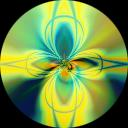
\includegraphics[width=0.16670in,height=0.16670in]{../ReversalLearning_20130621/images/abs4.jpg}
& 2.7 & PreReversal & 1 & Nonresponse &\tabularnewline
2
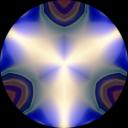
\includegraphics[width=0.16670in,height=0.16670in]{../ReversalLearning_20130621/images/abs2.jpg}
& 5.2 & Control & 1 & Correct & 522\tabularnewline
3
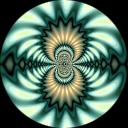
\includegraphics[width=0.16670in,height=0.16670in]{../ReversalLearning_20130621/images/abs3.jpg}
& 7.9 & PreReversal & 1 & Incorrect & 347\tabularnewline
1
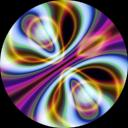
\includegraphics[width=0.16670in,height=0.16670in]{../ReversalLearning_20130621/images/abs1.jpg}
& 11.0 & Control & 1 & Incorrect & 595\tabularnewline
2
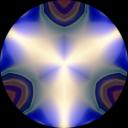
\includegraphics[width=0.16670in,height=0.16670in]{../ReversalLearning_20130621/images/abs2.jpg}
& 14.1 & Control & 2 & Correct & 720\tabularnewline
1
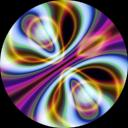
\includegraphics[width=0.16670in,height=0.16670in]{../ReversalLearning_20130621/images/abs1.jpg}
& 16.9 & Control & 2 & Incorrect & 580\tabularnewline
3
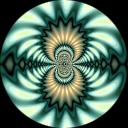
\includegraphics[width=0.16670in,height=0.16670in]{../ReversalLearning_20130621/images/abs3.jpg}
& 19.6 & PreReversal & 2 & Incorrect & 471\tabularnewline
4
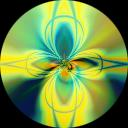
\includegraphics[width=0.16670in,height=0.16670in]{../ReversalLearning_20130621/images/abs4.jpg}
& 22.4 & PreReversal & 2 & Incorrect & 407\tabularnewline
1
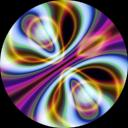
\includegraphics[width=0.16670in,height=0.16670in]{../ReversalLearning_20130621/images/abs1.jpg}
& 25.7 & Control & 3 & Correct & 641\tabularnewline
3
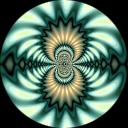
\includegraphics[width=0.16670in,height=0.16670in]{../ReversalLearning_20130621/images/abs3.jpg}
& 28.3 & PreReversal & 3 & Incorrect & 737\tabularnewline
4
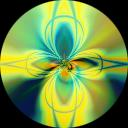
\includegraphics[width=0.16670in,height=0.16670in]{../ReversalLearning_20130621/images/abs4.jpg}
& 31.0 & PreReversal & 3 & Incorrect & 478\tabularnewline
2
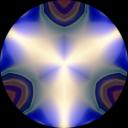
\includegraphics[width=0.16670in,height=0.16670in]{../ReversalLearning_20130621/images/abs2.jpg}
& 34.3 & Control & 3 & Incorrect & 778\tabularnewline
3
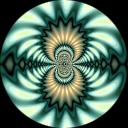
\includegraphics[width=0.16670in,height=0.16670in]{../ReversalLearning_20130621/images/abs3.jpg}
& 37.0 & PreReversal & 4 & Nonresponse &\tabularnewline
1
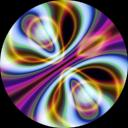
\includegraphics[width=0.16670in,height=0.16670in]{../ReversalLearning_20130621/images/abs1.jpg}
& 40.7 & Control & 4 & Incorrect & 563\tabularnewline
4
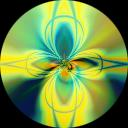
\includegraphics[width=0.16670in,height=0.16670in]{../ReversalLearning_20130621/images/abs4.jpg}
& 43.7 & PreReversal & 4 & Correct & 398\tabularnewline
2
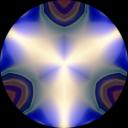
\includegraphics[width=0.16670in,height=0.16670in]{../ReversalLearning_20130621/images/abs2.jpg}
& 46.6 & Control & 4 & Correct & 650\tabularnewline
4
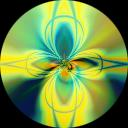
\includegraphics[width=0.16670in,height=0.16670in]{../ReversalLearning_20130621/images/abs4.jpg}
& 49.8 & PreReversal & 5 & Correct & 754\tabularnewline
2
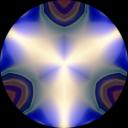
\includegraphics[width=0.16670in,height=0.16670in]{../ReversalLearning_20130621/images/abs2.jpg}
& 54.6 & Control & 5 & Correct & 595\tabularnewline
3
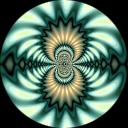
\includegraphics[width=0.16670in,height=0.16670in]{../ReversalLearning_20130621/images/abs3.jpg}
& 57.2 & PreReversal & 5 & Incorrect & 680\tabularnewline
5
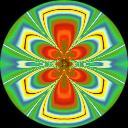
\includegraphics[width=0.16670in,height=0.16670in]{../ReversalLearning_20130621/images/abs5.jpg}
& 59.7 & PreReversal & 1 & Incorrect & 737\tabularnewline
1
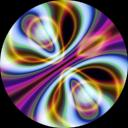
\includegraphics[width=0.16670in,height=0.16670in]{../ReversalLearning_20130621/images/abs1.jpg}
& 63.6 & Control & 5 & Incorrect & 534\tabularnewline
3
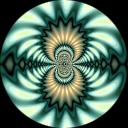
\includegraphics[width=0.16670in,height=0.16670in]{../ReversalLearning_20130621/images/abs3.jpg}
& 66.2 & PostReversal & 1 & Correct & 818\tabularnewline
4
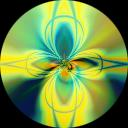
\includegraphics[width=0.16670in,height=0.16670in]{../ReversalLearning_20130621/images/abs4.jpg}
& 69.5 & PreReversal & 6 & Correct & 858\tabularnewline
6
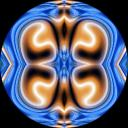
\includegraphics[width=0.16670in,height=0.16670in]{../ReversalLearning_20130621/images/abs6.jpg}
& 72.9 & PreReversal & 1 & Correct & 723\tabularnewline
3
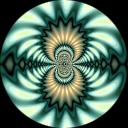
\includegraphics[width=0.16670in,height=0.16670in]{../ReversalLearning_20130621/images/abs3.jpg}
& 75.9 & PostReversal & 2 & Incorrect & 965\tabularnewline
4
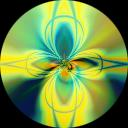
\includegraphics[width=0.16670in,height=0.16670in]{../ReversalLearning_20130621/images/abs4.jpg}
& 79.4 & PostReversal & 1 & Correct & 590\tabularnewline
6
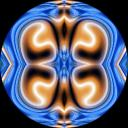
\includegraphics[width=0.16670in,height=0.16670in]{../ReversalLearning_20130621/images/abs6.jpg}
& 82.2 & PreReversal & 2 & Incorrect & 802\tabularnewline
4
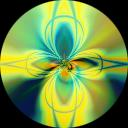
\includegraphics[width=0.16670in,height=0.16670in]{../ReversalLearning_20130621/images/abs4.jpg}
& 85.5 & PostReversal & 2 & Correct & 934\tabularnewline
5
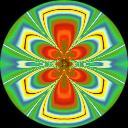
\includegraphics[width=0.16670in,height=0.16670in]{../ReversalLearning_20130621/images/abs5.jpg}
& 88.6 & PreReversal & 2 & Nonresponse &\tabularnewline
6
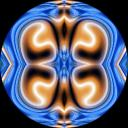
\includegraphics[width=0.16670in,height=0.16670in]{../ReversalLearning_20130621/images/abs6.jpg}
& 92.1 & PreReversal & 3 & Correct & 800\tabularnewline
4
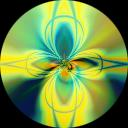
\includegraphics[width=0.16670in,height=0.16670in]{../ReversalLearning_20130621/images/abs4.jpg}
& 95.3 & PostReversal & 3 & Incorrect & 513\tabularnewline
5
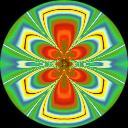
\includegraphics[width=0.16670in,height=0.16670in]{../ReversalLearning_20130621/images/abs5.jpg}
& 99.2 & PreReversal & 3 & Correct & 567\tabularnewline
3
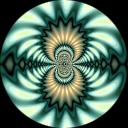
\includegraphics[width=0.16670in,height=0.16670in]{../ReversalLearning_20130621/images/abs3.jpg}
& 104.4 & PostReversal & 3 & Incorrect & 471\tabularnewline
4
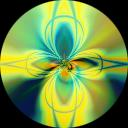
\includegraphics[width=0.16670in,height=0.16670in]{../ReversalLearning_20130621/images/abs4.jpg}
& 107.7 & PostReversal & 4 & Correct & 536\tabularnewline
6
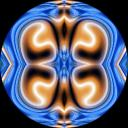
\includegraphics[width=0.16670in,height=0.16670in]{../ReversalLearning_20130621/images/abs6.jpg}
& 110.3 & PreReversal & 4 & Correct & 644\tabularnewline
5
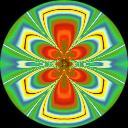
\includegraphics[width=0.16670in,height=0.16670in]{../ReversalLearning_20130621/images/abs5.jpg}
& 113.3 & PreReversal & 4 & Correct & 389\tabularnewline
3
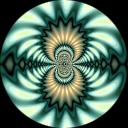
\includegraphics[width=0.16670in,height=0.16670in]{../ReversalLearning_20130621/images/abs3.jpg}
& 116.3 & PostReversal & 4 & Correct & 377\tabularnewline
5
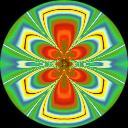
\includegraphics[width=0.16670in,height=0.16670in]{../ReversalLearning_20130621/images/abs5.jpg}
& 119.6 & PreReversal & 5 & Correct & 463\tabularnewline
3
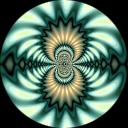
\includegraphics[width=0.16670in,height=0.16670in]{../ReversalLearning_20130621/images/abs3.jpg}
& 122.5 & PostReversal & 5 & Correct & 369\tabularnewline
4
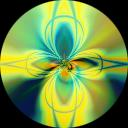
\includegraphics[width=0.16670in,height=0.16670in]{../ReversalLearning_20130621/images/abs4.jpg}
& 125.1 & PostReversal & 5 & Correct & 549\tabularnewline
\bottomrule
\end{longtable}

Last 40:

\begin{longtable}[]{@{}lrlrll@{}}
\toprule
Image & Onset (s) & Presentation Type & Image Presentation & Response &
RT (ms)\tabularnewline
\midrule
\endhead
20
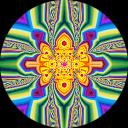
\includegraphics[width=0.16670in,height=0.16670in]{../ReversalLearning_20130621/images/abs20.jpg}
& 580.5 & PreReversal & 1 & Correct & 520\tabularnewline
18
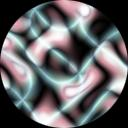
\includegraphics[width=0.16670in,height=0.16670in]{../ReversalLearning_20130621/images/abs18.jpg}
& 587.6 & PreReversal & 6 & Correct & 883\tabularnewline
19
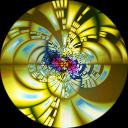
\includegraphics[width=0.16670in,height=0.16670in]{../ReversalLearning_20130621/images/abs19.jpg}
& 590.2 & PreReversal & 2 & Incorrect & 541\tabularnewline
17
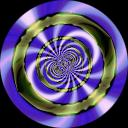
\includegraphics[width=0.16670in,height=0.16670in]{../ReversalLearning_20130621/images/abs17.jpg}
& 593.2 & PostReversal & 2 & Correct & 413\tabularnewline
18
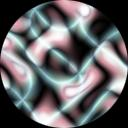
\includegraphics[width=0.16670in,height=0.16670in]{../ReversalLearning_20130621/images/abs18.jpg}
& 595.9 & PostReversal & 1 & Incorrect & 488\tabularnewline
20
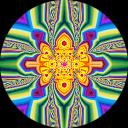
\includegraphics[width=0.16670in,height=0.16670in]{../ReversalLearning_20130621/images/abs20.jpg}
& 598.8 & PreReversal & 2 & Incorrect & 446\tabularnewline
18
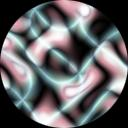
\includegraphics[width=0.16670in,height=0.16670in]{../ReversalLearning_20130621/images/abs18.jpg}
& 602.2 & PostReversal & 2 & Correct & 260\tabularnewline
20
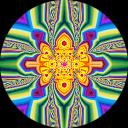
\includegraphics[width=0.16670in,height=0.16670in]{../ReversalLearning_20130621/images/abs20.jpg}
& 605.7 & PreReversal & 3 & Incorrect & 354\tabularnewline
19
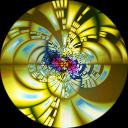
\includegraphics[width=0.16670in,height=0.16670in]{../ReversalLearning_20130621/images/abs19.jpg}
& 608.5 & PreReversal & 3 & Correct & 416\tabularnewline
18
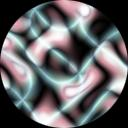
\includegraphics[width=0.16670in,height=0.16670in]{../ReversalLearning_20130621/images/abs18.jpg}
& 611.0 & PostReversal & 3 & Incorrect & 833\tabularnewline
17
\includegraphics[width=0.16670in,height=0.16670in]{../ReversalLearning_20130621/images/abs17.jpg}
& 616.0 & PostReversal & 3 & Incorrect & 394\tabularnewline
20
\includegraphics[width=0.16670in,height=0.16670in]{../ReversalLearning_20130621/images/abs20.jpg}
& 618.6 & PreReversal & 4 & Incorrect & 843\tabularnewline
18
\includegraphics[width=0.16670in,height=0.16670in]{../ReversalLearning_20130621/images/abs18.jpg}
& 621.4 & PostReversal & 4 & Correct & 352\tabularnewline
19
\includegraphics[width=0.16670in,height=0.16670in]{../ReversalLearning_20130621/images/abs19.jpg}
& 625.0 & PreReversal & 4 & Nonresponse &\tabularnewline
17
\includegraphics[width=0.16670in,height=0.16670in]{../ReversalLearning_20130621/images/abs17.jpg}
& 628.2 & PostReversal & 4 & Incorrect & 458\tabularnewline
18
\includegraphics[width=0.16670in,height=0.16670in]{../ReversalLearning_20130621/images/abs18.jpg}
& 632.1 & PostReversal & 5 & Incorrect & 346\tabularnewline
17
\includegraphics[width=0.16670in,height=0.16670in]{../ReversalLearning_20130621/images/abs17.jpg}
& 634.6 & PostReversal & 5 & Correct & 380\tabularnewline
19
\includegraphics[width=0.16670in,height=0.16670in]{../ReversalLearning_20130621/images/abs19.jpg}
& 637.2 & PreReversal & 5 & Incorrect & 749\tabularnewline
20
\includegraphics[width=0.16670in,height=0.16670in]{../ReversalLearning_20130621/images/abs20.jpg}
& 640.5 & PreReversal & 5 & Correct & 849\tabularnewline
22
\includegraphics[width=0.16670in,height=0.16670in]{../ReversalLearning_20130621/images/abs22.jpg}
& 643.7 & Control & 1 & Correct & 579\tabularnewline
19
\includegraphics[width=0.16670in,height=0.16670in]{../ReversalLearning_20130621/images/abs19.jpg}
& 646.9 & PostReversal & 1 & Correct & 452\tabularnewline
20
\includegraphics[width=0.16670in,height=0.16670in]{../ReversalLearning_20130621/images/abs20.jpg}
& 650.8 & PreReversal & 6 & Correct & 446\tabularnewline
21
\includegraphics[width=0.16670in,height=0.16670in]{../ReversalLearning_20130621/images/abs21.jpg}
& 656.4 & Control & 1 & Incorrect & 406\tabularnewline
22
\includegraphics[width=0.16670in,height=0.16670in]{../ReversalLearning_20130621/images/abs22.jpg}
& 663.5 & Control & 2 & Incorrect & 404\tabularnewline
20
\includegraphics[width=0.16670in,height=0.16670in]{../ReversalLearning_20130621/images/abs20.jpg}
& 666.7 & PreReversal & 7 & Correct & 720\tabularnewline
21
\includegraphics[width=0.16670in,height=0.16670in]{../ReversalLearning_20130621/images/abs21.jpg}
& 669.7 & Control & 2 & Incorrect & 671\tabularnewline
19
\includegraphics[width=0.16670in,height=0.16670in]{../ReversalLearning_20130621/images/abs19.jpg}
& 672.7 & PostReversal & 2 & Incorrect & 357\tabularnewline
20
\includegraphics[width=0.16670in,height=0.16670in]{../ReversalLearning_20130621/images/abs20.jpg}
& 675.6 & PostReversal & 1 & Incorrect & 554\tabularnewline
19
\includegraphics[width=0.16670in,height=0.16670in]{../ReversalLearning_20130621/images/abs19.jpg}
& 678.8 & PostReversal & 3 & Incorrect & 436\tabularnewline
21
\includegraphics[width=0.16670in,height=0.16670in]{../ReversalLearning_20130621/images/abs21.jpg}
& 681.3 & Control & 3 & Incorrect & 380\tabularnewline
20
\includegraphics[width=0.16670in,height=0.16670in]{../ReversalLearning_20130621/images/abs20.jpg}
& 684.2 & PostReversal & 2 & Incorrect & 227\tabularnewline
22
\includegraphics[width=0.16670in,height=0.16670in]{../ReversalLearning_20130621/images/abs22.jpg}
& 687.4 & Control & 3 & Incorrect & 267\tabularnewline
20
\includegraphics[width=0.16670in,height=0.16670in]{../ReversalLearning_20130621/images/abs20.jpg}
& 690.0 & PostReversal & 3 & Correct & 301\tabularnewline
21
\includegraphics[width=0.16670in,height=0.16670in]{../ReversalLearning_20130621/images/abs21.jpg}
& 692.7 & Control & 4 & Correct & 411\tabularnewline
19
\includegraphics[width=0.16670in,height=0.16670in]{../ReversalLearning_20130621/images/abs19.jpg}
& 695.6 & PostReversal & 4 & Incorrect & 379\tabularnewline
20
\includegraphics[width=0.16670in,height=0.16670in]{../ReversalLearning_20130621/images/abs20.jpg}
& 699.1 & PostReversal & 4 & Incorrect & 356\tabularnewline
22
\includegraphics[width=0.16670in,height=0.16670in]{../ReversalLearning_20130621/images/abs22.jpg}
& 701.9 & Control & 4 & Incorrect & 451\tabularnewline
20
\includegraphics[width=0.16670in,height=0.16670in]{../ReversalLearning_20130621/images/abs20.jpg}
& 705.1 & PostReversal & 5 & Correct & 480\tabularnewline
22
\includegraphics[width=0.16670in,height=0.16670in]{../ReversalLearning_20130621/images/abs22.jpg}
& 708.1 & Control & 5 & Incorrect & 411\tabularnewline
19
\includegraphics[width=0.16670in,height=0.16670in]{../ReversalLearning_20130621/images/abs19.jpg}
& 713.8 & PostReversal & 5 & Incorrect & 595\tabularnewline
21
\includegraphics[width=0.16670in,height=0.16670in]{../ReversalLearning_20130621/images/abs21.jpg}
& 716.9 & Control & 5 & Incorrect & 488\tabularnewline
\bottomrule
\end{longtable}

\section{Hierarchy}\label{hierarchy}

In order to model the RL task hierarchically it is important to grasp
the levels we need to model. These are:

\begin{itemize}
\tightlist
\item
  Subjects are organized into three groups, with around 50 subjects per
  group. The groups are Safe Sex, Risky Sex No Meth, and Risky Sex Meth.
  Between-group comparisons may have interesting implications for sexual
  health or drug abuse research.
\item
  There are two types of sessions, Reward and Punishment. Most subjects
  have done two sessions of each, i.e., four sessions per subject.
  However, there's quite a lot of missing data. Overall, 133 subjects
  have four sessions, 8 have three sessions (all of which include both a
  punishment and a reward session), and 14 subjects have only two
  sessions (4 of which are subjects with only reward sessions; 10 are
  subjects with only punishment sessions).
\end{itemize}


\end{document}
